% Part 2 §2.12 chapter carrying "Electroweak Symmetry Breaking and the Matter Sector" (Mar/Oct 2026), "Electron Rest Mass from Holographic Horizon
% Thermodynamics" (Feb 2026) and "Three Charged Lepton Generations and the Koide Ratio" (22 Apr 2026). All read in full 2026-10-02 (207, 485, 846 lines).
% Numbers: docs/verification/scripts/verify_electron_mass.py, verify_koide.py. Checks: docs/verification/particle/*_CHECK.md.
\chapter{The particle scale}\label{ch:particle}

\section*{The place}
IAM's Law (Chapter~\ref{ch:iams_law}) prices a classical record at $k_BT\ln2$ per bit on the nearest encoding surface, at that surface's temperature,
$T=\hbar\kappa/2\pi k_B$ for surface gravity $\kappa$. This chapter takes the law to the smallest scale at which it has been applied: the particles that
make up the matter sector. Three questions are asked: when a matter sector first exists, whether the electron's mass can be read as a fixed point of the
law, and whether the pattern of the charged-lepton masses follows from information partition on a surface.

\section{When the matter sector begins}
The criterion that divides the sectors is proper time: a degree of freedom decoheres gravitationally only if it accumulates proper time, $\Delta\tau>0$.
Above the electroweak scale the Higgs expectation value vanishes and the $W$, $Z$ and fermions have no rest mass; their excitations travel on null
geodesics. At $T\approx160$\,GeV~\cite{DOnofrio2016} the Higgs field takes its vacuum value $v=246$\,GeV, the $W^\pm$ and $Z^0$ acquire mass~\cite{Englert1964,Higgs1964}, the charged fermions acquire
$m_f=y_fv/\sqrt2$, and their excitations move on timelike worldlines. The matter sector exists from this epoch~\cite{MahaffeyEWSB}. The electromagnetic $U(1)$ survives
unbroken, so the photon stays exactly massless ($m_\gamma<10^{-18}$\,eV~\cite{PDG2022}) and on null geodesics: the photon's exemption from writing is a consequence
of an established gauge symmetry, not an added assumption. It does not by itself establish $\Sigma=1$, which is a statement about how the metric
potentials respond to matter and is tested by weak lensing.

The activation of the term comes much later. $E(a)=e^{1-1/a}$ is $\sim e^{-10^{15}}$ at the electroweak epoch, $9\times10^{-14}$ at $z=30$, $4.5\times10^{-5}$
at $z=10$ and $0.37$ at $z=1$: the matter sector exists from the electroweak epoch, and it writes in quantity only once structure forms.

The coupling divides between the two kinds of matter: $\beta_m=\Omega_b/2+\Omega_{\rm dm}/2=0.0247+0.1330=0.1577$ with Planck 2018 values~\cite{Planck2018VI}: $15.6\,\%$
baryonic, set by the baryon asymmetry (Chapter~\ref{ch:baryon}), and $84.4\,\%$ dark, set by the dark-matter density. Both are measured inputs.

The weak interaction forms no bound states and the strong interaction's confining potential is linear~\cite{Eichten1978}, not $1/r$; hadrons are virialised in their own
potential. The virial half that sets how much bound matter writes (Chapter~\ref{ch:virial}) applies to the $1/r$ interactions, gravity and electrostatics.

Open: whether the selection of the Higgs vacuum, a superposition over a degenerate manifold resolving into one classical vacuum, is itself a record
written at the temperature of the transition. Nothing in the cosmology depends on it.

\section{The electron as a fixed point}

\begin{figure}[htbp]\centering
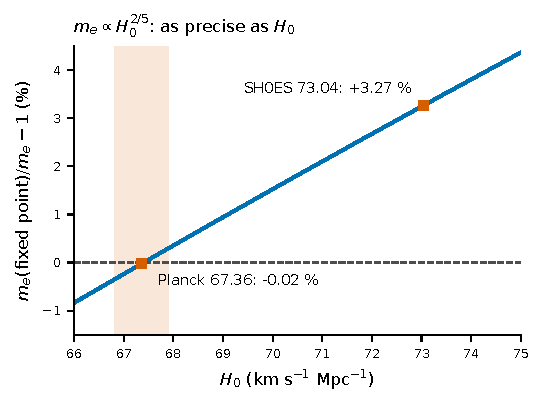
\includegraphics[width=0.62\textwidth]{figures/part2/fig_electron_h0.pdf}
\caption{The electron fixed point, $m_e\propto H_0^{2/5}$, against $H_0$: $-0.02\,\%$ at the Planck 67.36 (band: $\pm0.54$, which alone is $\pm0.32\,\%$ in $m_e$) and $+3.27\,\%$ at the SH0ES 73.04. CODATA 2018; \texttt{docs/verification/scripts/\allowbreak{}verify\_electron\_mass.py}. One factor, $(2\pi)^{3/10}$, is identified numerically. \calc}\label{fig:electron_h0}
\end{figure}
The same temperature formula serves a black-hole horizon ($\kappa=c^3/4GM$) and the cosmic horizon ($\kappa=H_0$). The electron paper~\cite{MahaffeyElectron} asks whether the
electron's rest energy is the cost of maintaining its own record, written at the cosmic horizon's temperature:
\begin{equation}mc^2=E_{\rm bit}\,\frac{N(m)}{f(\alpha)},\qquad E_{\rm bit}=k_BT_{GH}\ln2=\frac{\hbar H_0\ln2}{2\pi}.\end{equation}
Three ingredients enter, each stated as an assumption: the Compton sphere $\bar\lambda_C=\hbar/mc$ saturates the Bekenstein bound~\cite{Bekenstein1981},
$S=\pi(m_P/m)^2$; the number of encoding cells scales as $N\propto(m_P/m)^{3/2}$, argued from dimensional homogeneity and the virial scaling of a
$1/r$ potential; and the electromagnetic self-energy suppresses the gravitational channel by $f(\alpha)=\alpha^{5/2}$, obtained two ways --- spatially,
as the occupied fraction of phase-space cells $(r_e/\bar\lambda_C)^{3/2}=\alpha^{3/2}$ times the diverted energy fraction $\alpha$; and temporally, as
the dilution $\alpha$ of the gravitational clock times the phase-space volume $\alpha^{3/2}$ of the electromagnetic orbit. $m$ appears on both sides, so the
condition is a fixed point:
\begin{equation}m_e=(2\pi)^{-1/10}\left[\frac{\hbar H_0\ln2\;m_P^{3/2}}{\alpha^{5/2}c^2}\right]^{2/5}.\end{equation}
\paragraph{What the numbers show.} Without the prefactor the bracket gives $1.2018\,m_e$. The factor $(2\pi)^{-1/10}=0.832112$ was found by search
among clean combinations of constants; $(2\pi)^{-2/5}$ of it follows from $T_{GH}$ through the $2/5$ root, and the remaining $(2\pi)^{3/10}$ has no
derivation (a proposed origin is the quarter of the Euclidean thermal circle traversed by the null geodesic from the Compton sphere to the de Sitter
horizon). The result scales as $m_e\propto H_0^{2/5}$, so its precision is that of $H_0$: the Planck uncertainty $\sigma(H_0)=0.54$~\cite{Planck2018VI} alone is $\pm0.32\,\%$
in $m_e$. With $H_0=67.4$ the deviation is $+6.6$\,ppm; with the Planck best value $67.36$ it is $-231$\,ppm; with $73.0$ it is $+3.3\,\%$. Stated
at the precision the inputs allow: the fixed point lands on the electron mass to within the $0.3\,\%$ set by $H_0$, with one factor identified
numerically.
\paragraph{Constancy.} $H_0$ enters as today's value: the fixed point is read off the present horizon and does not predict a drift of $m_e$; quasar
spectra bound $\Delta(m_p/m_e)/(m_p/m_e)<10^{-5}$. Why the present horizon, rather than one co-evolving with $H(t)$, is open, and the proton, a composite,
is not treated.
\paragraph{The black hole.} For a Schwarzschild horizon the bits priced at $k_BT_H\ln2$ total $\tfrac12Mc^2$ (Smarr~\cite{Smarr1973}; Chapter~\ref{ch:blackholes}),
not $Mc^2$: the two horizons share the temperature formula, but the black hole closes with the virial half.

\section{The charged-lepton pattern}

\begin{figure}[htbp]\centering
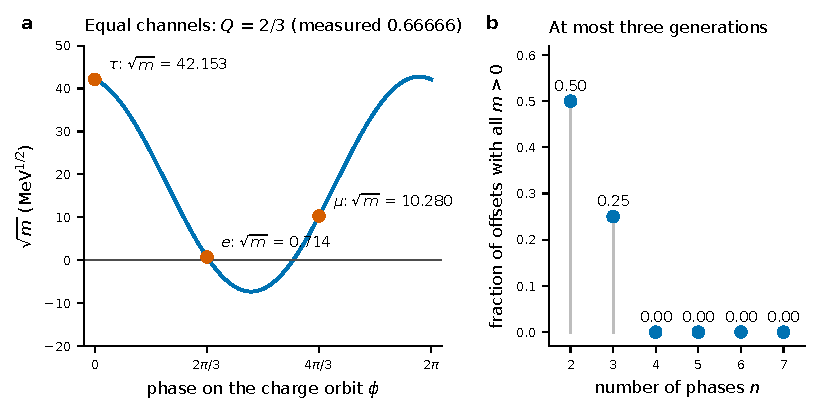
\includegraphics[width=\textwidth]{figures/part2/fig_koide.pdf}
\caption{(a) The encoding $\sqrt{m(\phi)}=x(1+\sqrt2\cos(\phi+\delta))$ with $x^2=313.84$\,MeV and $\delta=0.22227$\,rad fixed by the measured pole masses; the three phases $2\pi k/3$ return $\sqrt{m}$ of the $\tau$, $e$ and $\mu$ ($Q=0.66666051$) \observed. (b) The fraction of offsets $\delta$ for which all $n$ masses are positive with $y/x=\sqrt2$: 0.50 for $n=2$, 0.25 for $n=3$, none for $n\ge4$. \calc}\label{fig:koide}
\end{figure}
The charged-lepton pole masses satisfy Koide's relation~\cite{Koide1982,Koide1983}
\begin{equation}Q=\frac{m_e+m_\mu+m_\tau}{(\sqrt{m_e}+\sqrt{m_\mu}+\sqrt{m_\tau})^2}=0.66666051\end{equation}
($2/3$ to $10^{-5}$), which has no Standard Model derivation. Write the square roots as one encoding on a charge orbit $S^1$~\cite{MahaffeyKoide},
$\sqrt{m(\phi)}=x+y\cos(\phi+\delta)$, sampled at $n$ equally spaced phases. The constant mode and the first harmonic are independent channels, with
orbit-averaged weights $x^2$ and $y^2/2$; higher harmonics cost gradient energy $\propto n^2$ and are absent in the ground state. If the boundary
partitions information equally between independent channels --- the maximum-entropy partition, the same principle that makes the Bekenstein--Hawking
entropy the bound --- then $x^2=y^2/2$, $y/x=\sqrt2$, and for $n=3$
\begin{equation}\sum_k\sqrt{m_k}=3x,\qquad\sum_km_k=3x^2+\tfrac32y^2,\qquad Q=\tfrac13\Big(1+\frac{y^2}{2x^2}\Big)=\tfrac23\end{equation}
exactly, for every $\delta$.
\paragraph{How many generations.} With $y/x=\sqrt2$ every mass must satisfy $1+\sqrt2\cos\phi_k>0$. For four or more phases this fails for every
offset $\delta$: one phase always lies within $\pi/4$ of $\pi$. So equipartition allows at most three generations. Two generations are allowed for half
of all offsets, so "exactly three" is not derived.
\paragraph{The offset.} The measured masses~\cite{PDG2022} fix $x^2=313.84$\,MeV and $\delta=0.22227$\,rad (close to $2/9$, Brannen 2006~\cite{Brannen2006}), which reproduce
$m_e=0.510$ and $m_\mu=105.68$\,MeV from $m_\tau$. With $\delta=0$ the two lighter masses would be equal ($26.9$\,MeV each). The offset and the scale $x$
are not derived.
\paragraph{Assumptions.} The reduction of a fixed-charge sector to an $S^1$ orbit is taken from the gauge/global correspondence, on firm footing in
AdS/CFT~\cite{Maldacena1999} and an open question in de Sitter. Koide's relation holds for pole masses and degrades under running~\cite{Xing2006}; why the pole masses is open.

\section{Status}
Stands: the matter sector begins with electroweak symmetry breaking and the photon stays outside it by an exact symmetry; equipartition on a charge
orbit gives $Q=2/3$ and at most three generations. Measured here: the electron fixed point reaches $m_e$ within the $0.3\,\%$ allowed by $H_0$ with one
numerically identified factor. Open: the $(2\pi)^{3/10}$ factor; the Koide offset $\delta$ and scale $x$; why exactly three and not two.
